\documentclass[presentation]{beamer}
\usepackage{oop-slides}
\setbeamertemplate{bibliography item}[text]
\newcommand{\lessonnr}[0]{06}
\title[OOP\lessonnr{} -- Advanced Collections]{\lessonnr{}\\ Static code analysis, collezioni avanzate, enumeration e classi nested}

\begin{document}
	
\frame[label=coverpage]{\titlepage}

%====================
%Outline
%====================
\newcommand{\al}[0]{\textless}
\newcommand{\ar}[0]{\textgreater}
\newcommand{\gen}[1]{\al{}#1\ar{}}
\newcommand{\imgfr}[4]{\fr{#1}{#2
\begin{center}
\includegraphics[width=#3\textwidth]{#4}                    
\end{center}
}}

\section{JAR e gestione del classpath in Eclipse}

\fr{Aggiunta di un jar al classpath di un progetto Eclipse - I} {
\bl{} {
		lab06 $\rightarrow$ Properties $\rightarrow$ Java build path $\rightarrow$ Libraries $\rightarrow$ Add Jar
	}
	\centering
	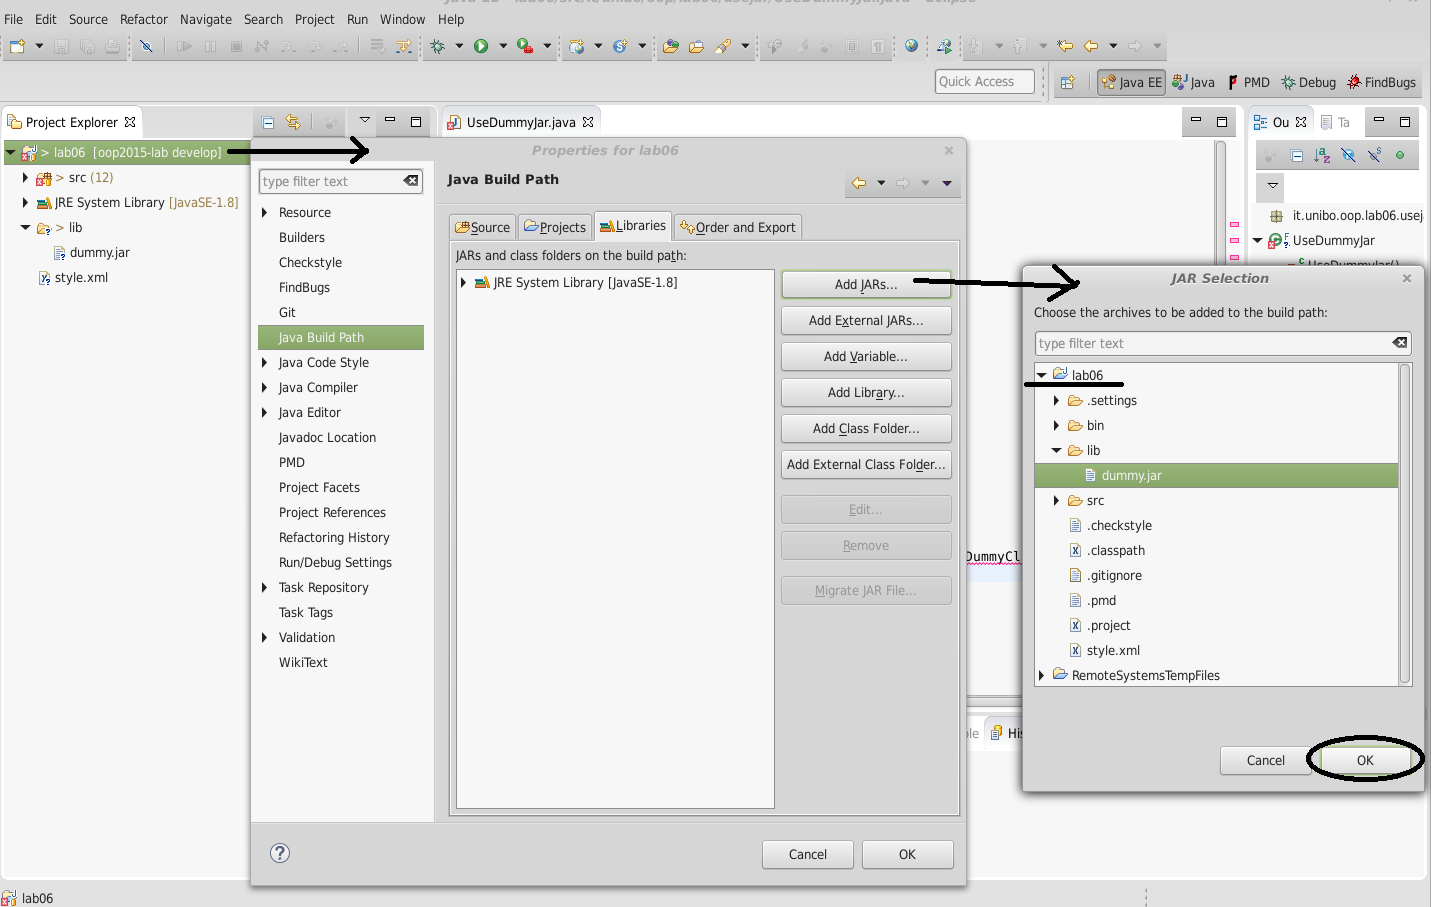
\includegraphics[width=0.99\textwidth]{img/addjar-1}
}

\fr{Aggiunta di un jar al classpath di un progetto Eclipse - II} {
	\centering
	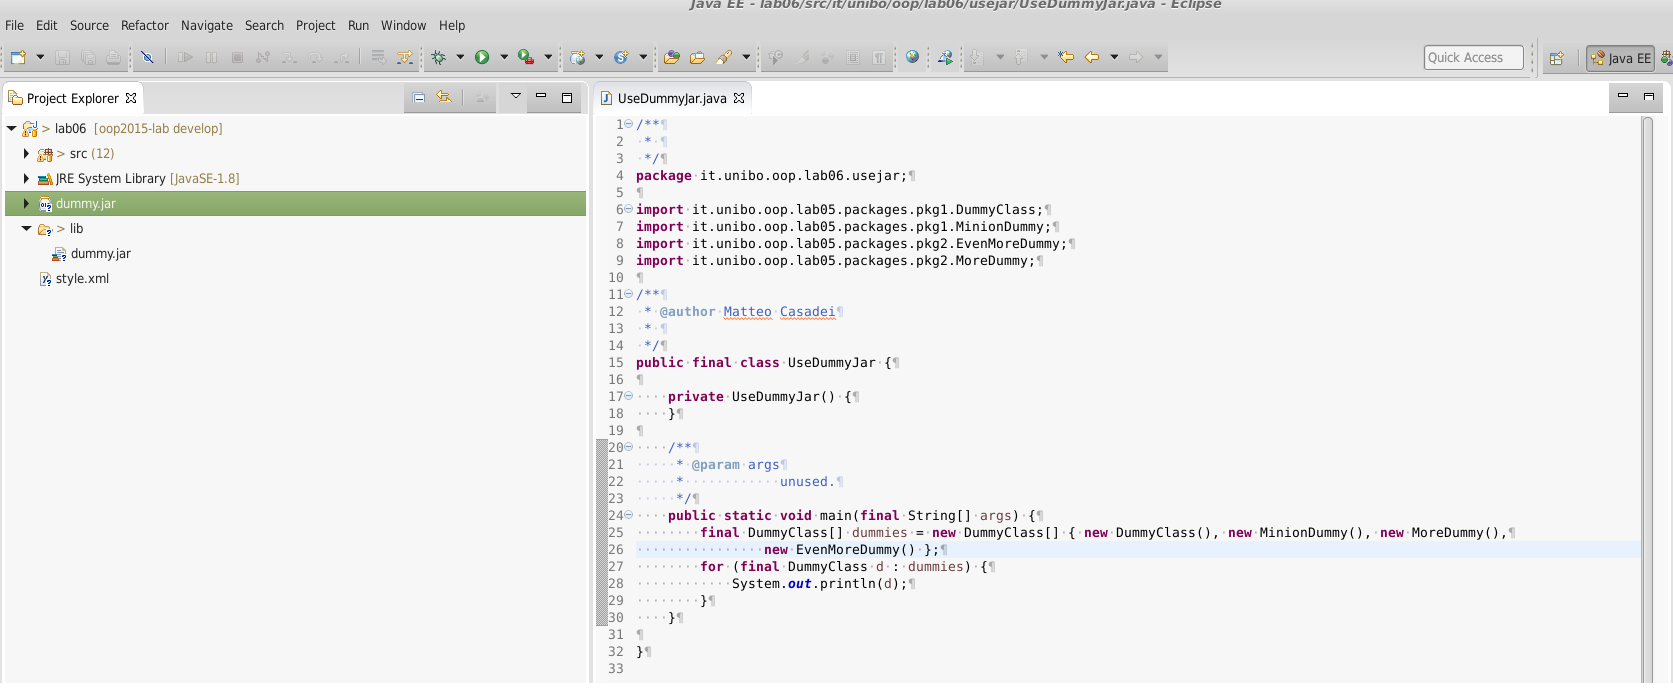
\includegraphics[width=0.99\textwidth]{img/addjar-2}
}

\fr{Aggiunta di un jar al classpath di un progetto Eclipse - III} {
	\centering
	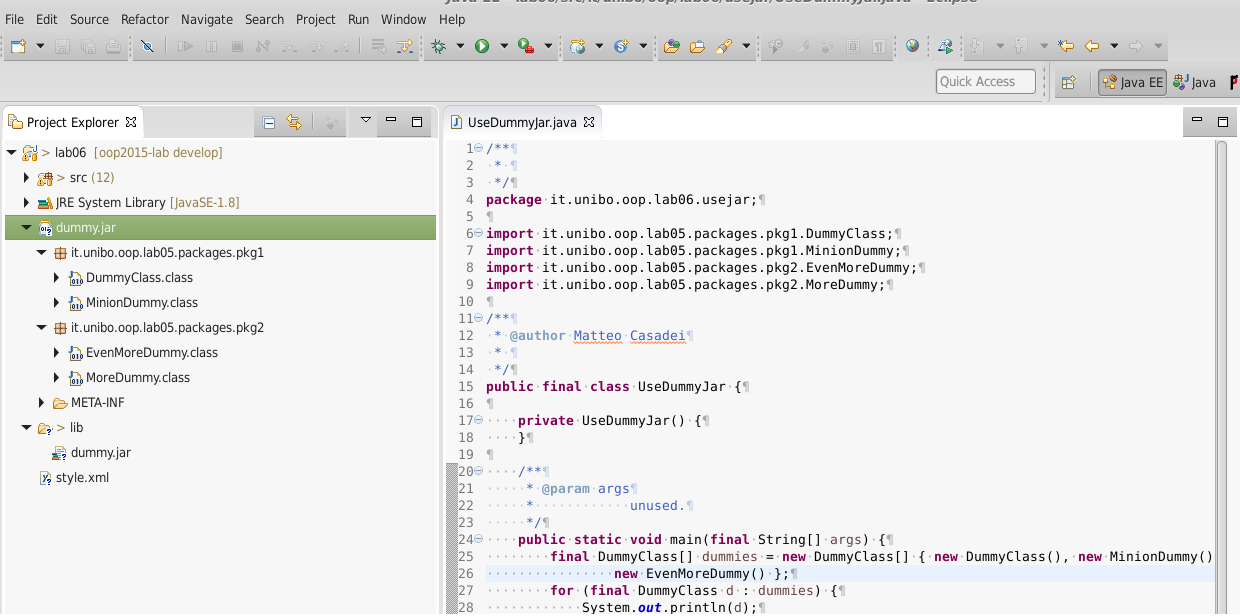
\includegraphics[width=0.99\textwidth]{img/addjar-3}
}

\section{Static source code analysis}

\fr{Static source code analysis} {
	\bl{Cos'è} {
		Utilizzo di software in grado di analizzare staticamente (senza che venga compilato od eseguito) del sorgente Java, per scoprire:
		\iz {
			\item Potenziali bug, magari dovuti a distrazione
			\item Possibili miglioramenti, ottimizzazioni o pratiche difformi da quelle consigliate
			\item Codice duplicato, segnale di una progettazione discutibile
			\item Stile non coerente, specie se si lavora in più persone su un progetto
		}
	}
	\bl{Utilità} {
		L'analisi automatica del proprio codice garantisce sempre un elevata qualità del codice, aiuta ad apprendere il modo corretto di scrivere, riduce il costo di manutenzione e garantisce uniformità fra le parti sviluppate da persone diverse.
	}
}

\subsection{FindBugs}

\fr{FindBugs} {
	\bl{Cos'è} {
		FindBugs si occupa di trovare potenziali bug nel sorgente, ad esempio:
		\iz {
			\item Uguaglianza esatta fra \texttt{float} o \texttt{double}
			\item Utilizzo di \texttt{==} invece di \texttt{equals()}
			\item Mancato retain a runtime di annotazioni
			\item Uso errato di meccanismi di sincronizzazione
			\item Vulnerabilità di sicurezza
			\item Tanti altri! Si veda: \url{http://findbugs.sourceforge.net/bugDescriptions.html}
		}
	}
}

\fr{FindBugs} {
	\bl{Plugin Eclipse} {
		Può essere installato dal marketplace di Eclipse cercando ``findbugs''.
		
		Una volta installato, apparirà un nuovo sotto-menu del progetto:
		
		\centering
		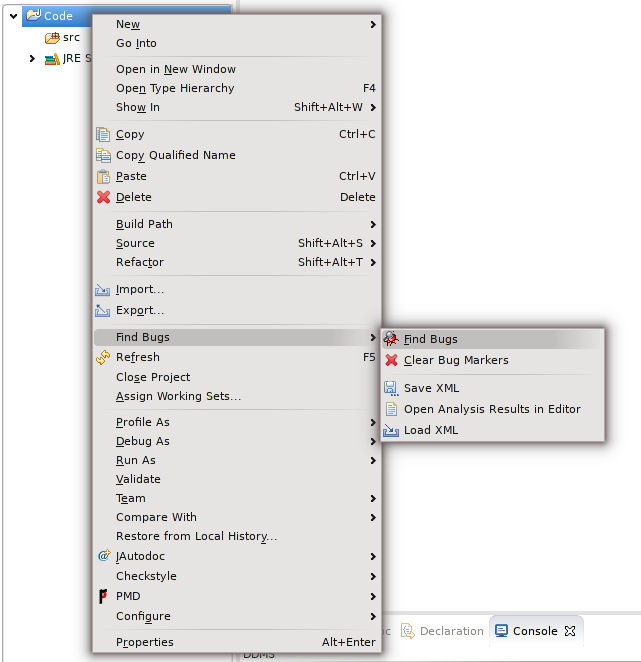
\includegraphics[width=0.5\textwidth]{img/findbugs}
	}
}

\fr{FindBugs --- Configurazione globale} {
	\centering
	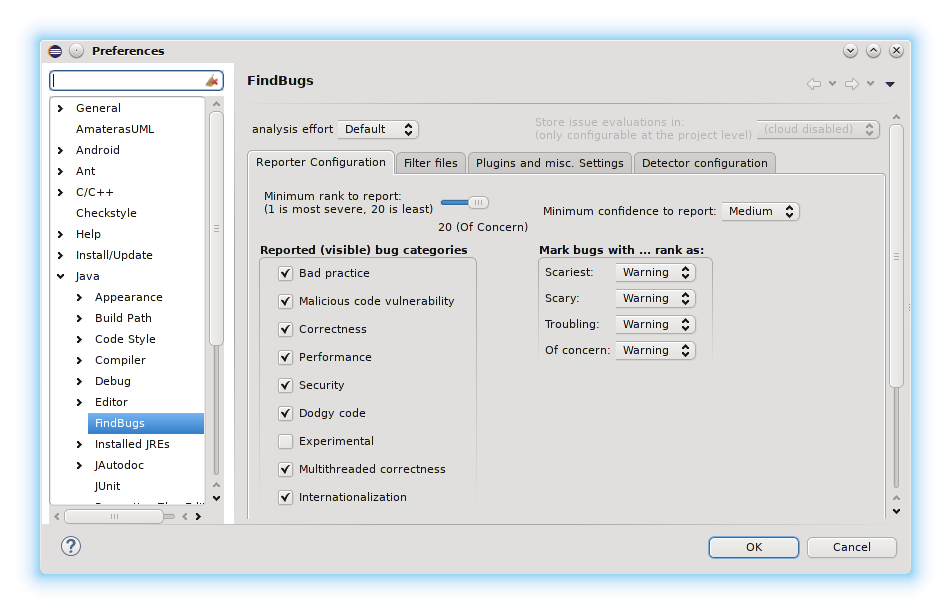
\includegraphics[width=0.99\textwidth]{img/findbugsconf}
}

\fr{FindBugs --- Configurazione del progetto} {
	\centering
	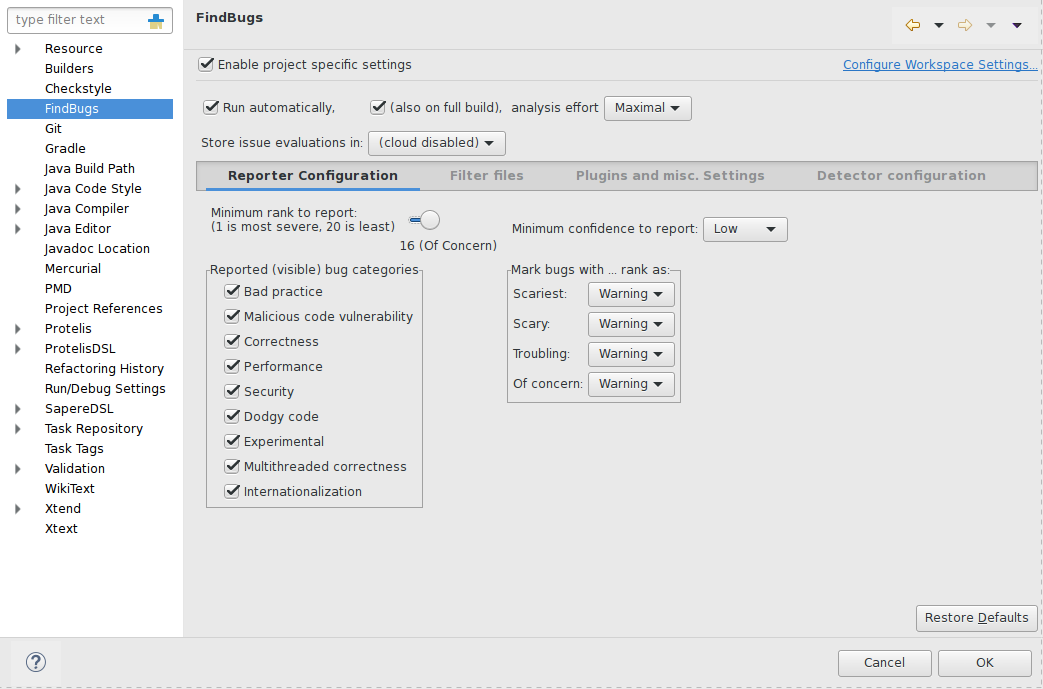
\includegraphics[width=0.9\textwidth]{img/findbugsproj}
}

\subsection{PMD e CPD}
\fr{PMD e CPD} {
	\bl{Cos'è} {
		PMD si occupa di trovare imperfezioni nel codice:
		\iz {
			\item Campi protetti o default
			\item Mancato uso di final
			\item Singular fields
			\item Usa CPD per verificare se vi siano blocchi di codice copincollati
			\item Tanti altri! Si veda: \url{http://pmd.sourceforge.net/pmd-4.3.0/rules/index.html}
		}
	}
}

\fr{PMD} {
	\bl{Plugin Eclipse --- installazione} {
		Il marketplace contiene due plugin concorrenti: meglio eseguire l'installazione manuale.
		\iz {
			\item Dal menu Help, si selezioni ``Install new software''
			\item Si incolli l'indirizzo \url{https://sourceforge.net/projects/pmd/files/pmd-eclipse/update-site-latest/} e si prema Enter
			\item Si selezioni ``PMD for Eclipse 4''
			\item Next, Finish
			\item Si accetti il codice non firmato
			\item Si riavvii Eclipse come suggerito
		}
	}
	\bl{Plugin Eclipse} {
		Al termine dell'installazione, verrà installato un menu di opzioni globali, un menu di opzioni per progetto ed un menu contestuale.
	}
}

\fr{PMD --- Configurazione globale} {
	La configurazione di default di PMD contiene regole con limiti arbitrari, regole che hanno senso solo in particolari environment (e.g. J2EE) e regole controverse. È meglio rimuovere tali regole!
	\iz{
		\item Dalle proprietà di Eclipse, si allarghi il sotto menu PMD
		\item Si vada su Rule Configuration
		\item Si selezionino tutte le regole (click su una, poi ctrl+A)
		\item Si eliminino tutte le regole
		\item Si usi il tasto import
		\item Si importino (meglio per copia) le regole da un file XML
		\item Vi forniremo noi un buon file di regole!
	}
}

\fr{PMD --- Configurazione globale} {
	\centering
	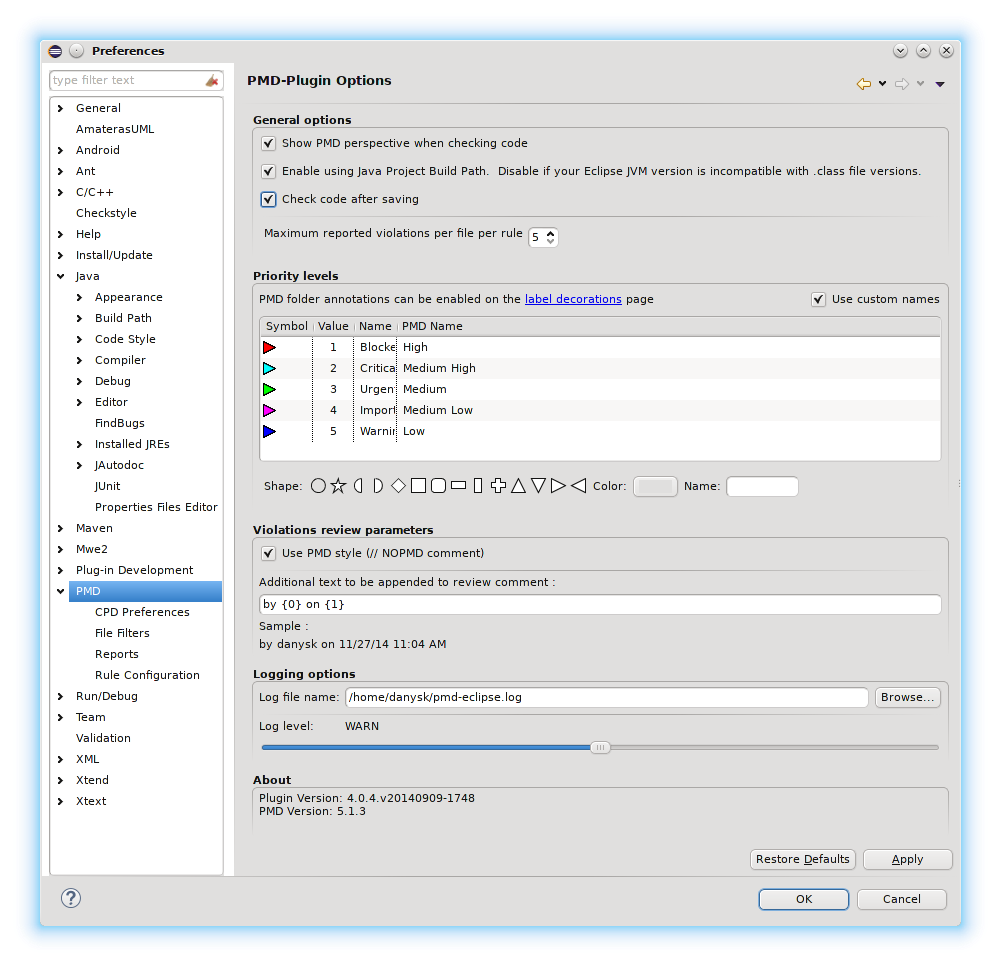
\includegraphics[width=0.75\textwidth]{img/pmdconf}
}

\fr{PMD --- Configurazione globale} {
	\centering
	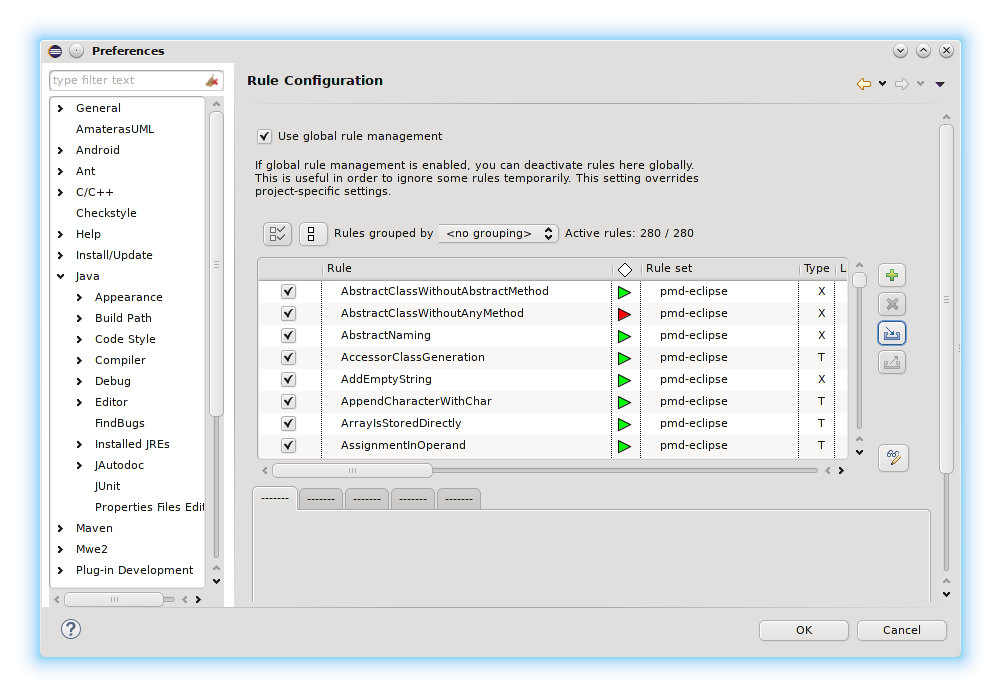
\includegraphics[width=0.99\textwidth]{img/pmdconf1}
}

\fr{PMD --- Configurazione globale} {
	\centering
	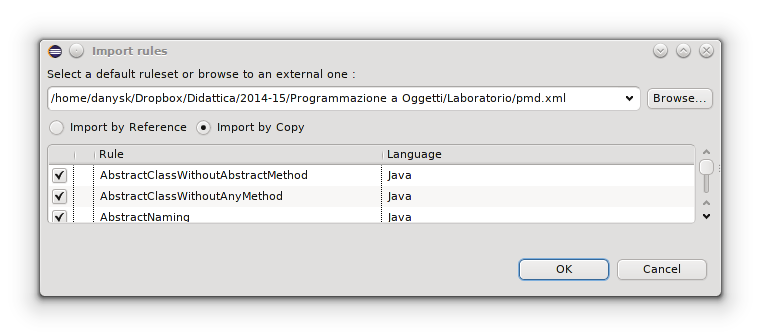
\includegraphics[width=0.99\textwidth]{img/pmdimport}
}

\fr{PMD --- Configurazione del progetto} {
	\centering
	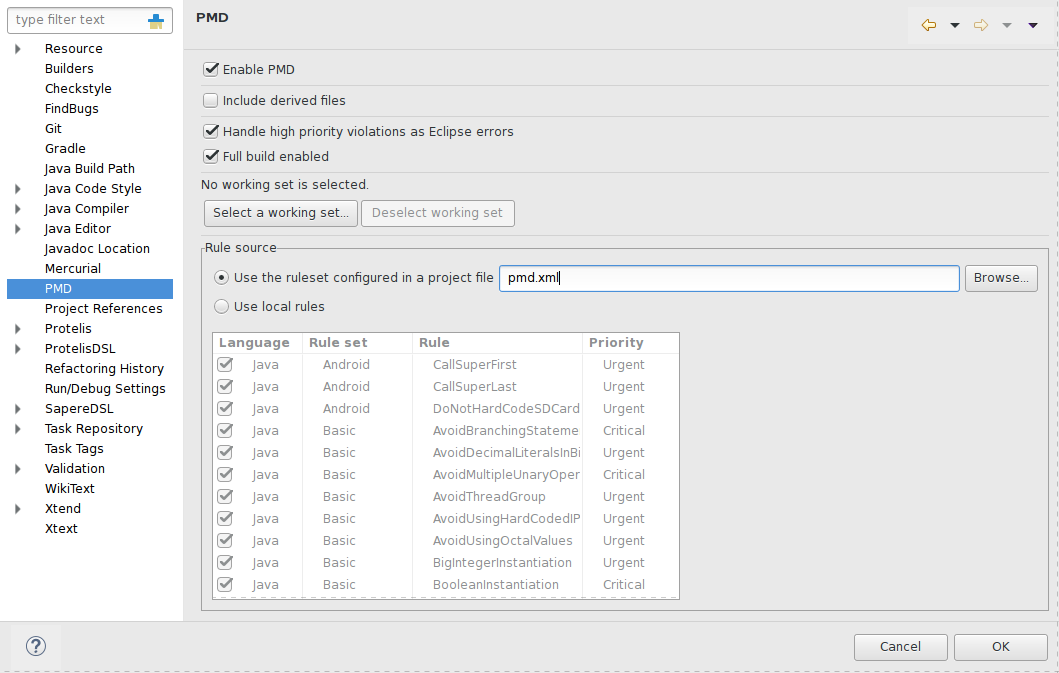
\includegraphics[width=0.99\textwidth]{img/pmdproj}
}


\subsection{Checkstyle}

\fr{Checkstyle} {
	\bl{Cos'è} {
		Checkstyle si occupa di trovare errori di stile:
		\iz {
			\item Mancanza di commento Javadoc
			\item Spaziature non corrette
			\item Parentesi assenti
			\item Magic numbers
			\item Altro: \url{http://checkstyle.sourceforge.net/checks.html}
		}
	}
}

\fr{Checkstyle} {
	\bl{Plugin Eclipse --- installazione} {
		Può essere installato dal marketplace di Eclipse cercando ``checkstyle plug-in''. Se si cerca solo ``checkstyle'', il primo risultato \textbf{non} è quello corretto. Il logo corretto presenta la scritta ``eclipse-cs''.

		Al termine dell'installazione, verrà installato un menu di opzioni globali, un menu di opzioni per progetto ed un menu contestuale.
	}
}

\fr{Checkstyle --- Configurazione globale} {
	La configurazione di default di Checkstyle è inadatta all'uso con Eclipse. C'è una configurazione built-in adatta ad Eclipse ma è eccessivamente pedante. Vi forniremo noi un file di configurazione per Checkstyle:
	\iz{
		\item Dalle proprietà di Eclipse, clicki sul menu Checkstyle
		\item Si vada su Rule Configuration
		\item Si scelga ``New''
		\item Si scelga ``Project Relative Configuration'' (mai usare path assoluti!)
		\item Utilizzando ``Browse...'' si punti al file di configurazione, che deve esser copiato nel progetto
		\item Si dia un nome e si prema ``OK''
		\item Si selezioni dalla lista la nuova Check configuration
		\item Si faccia click ``Set as Default''
	}
}

\fr{Checkstyle --- Configurazione globale} {
    Windows $\rightarrow$ Preferences $\rightarrow$ Java $\rightarrow$ Code style $\rightarrow$ Formatter
	\centering
	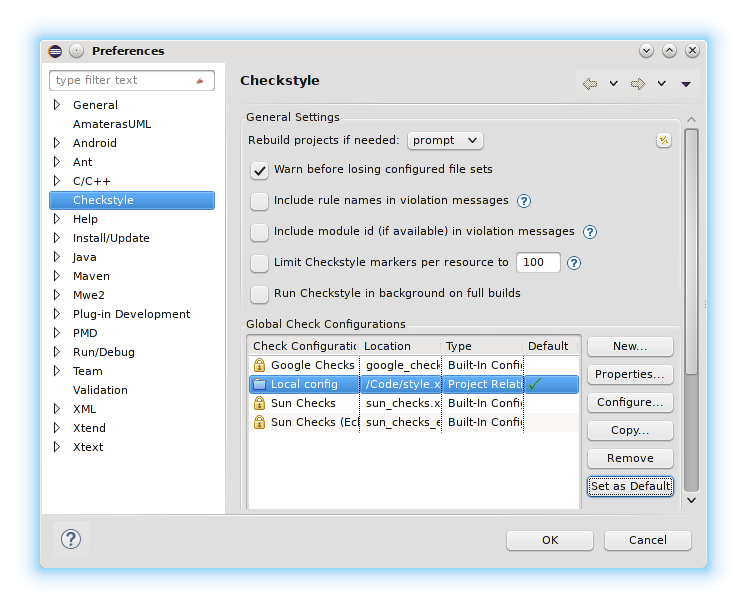
\includegraphics[width=0.9\textwidth]{img/checkstyleconf}
}

\fr{Checkstyle --- Configurazione del progetto} {
	\centering
	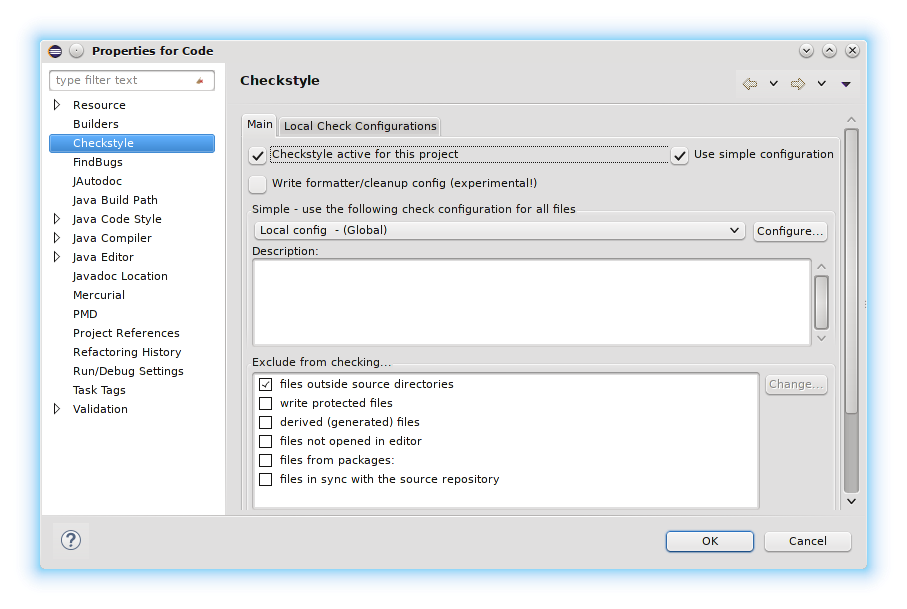
\includegraphics[width=0.99\textwidth]{img/checkstyleproj}
}

\section{Coding style: configurazione IDE Eclipse}
\fr{Configurare l'editor per una corretta formattazione del codice} {
	\bl{}{Checkstyle è in grado di supportarci nel verificare l'utilizzo di un corretto stile di codifica. Ovvero, seguendo la ``Java Code Convention'':
	\iz{
		\item 4 spazi per l'indentazione (NO TAB)
		\item Linee lunghe max 80 caratteri (meglio comunque 120!)
	}}
    \bl{}{Ora, però, dobbiamo configurare l'editor perché ci supporti nella scrittura di codice con lo stile corretto: come fare?}
}

\fr{Coding style: configurazione IDE Eclipse} {
	\centering
	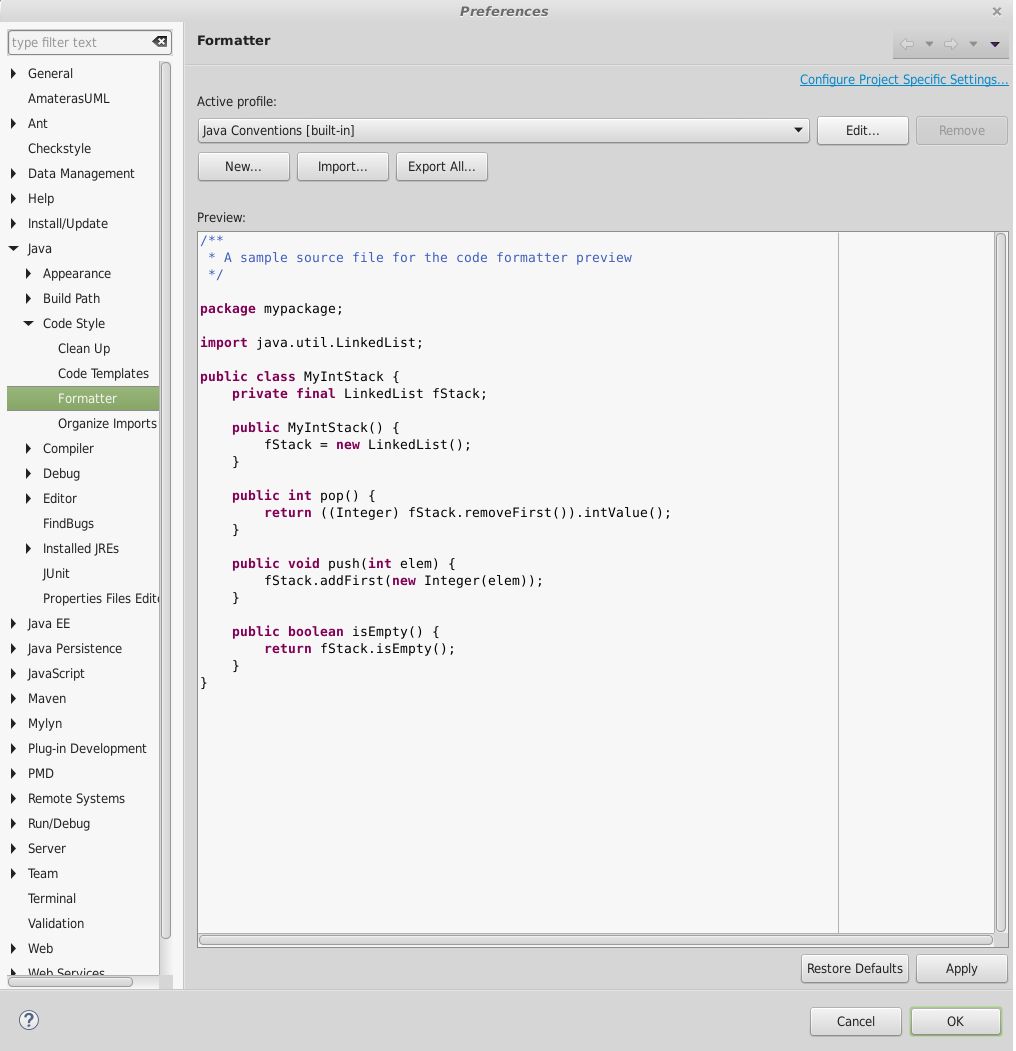
\includegraphics[width=0.99\textwidth]{img/ideconf-1}
}

\fr{Coding style: configurazione IDE Eclipse} {
	\centering
	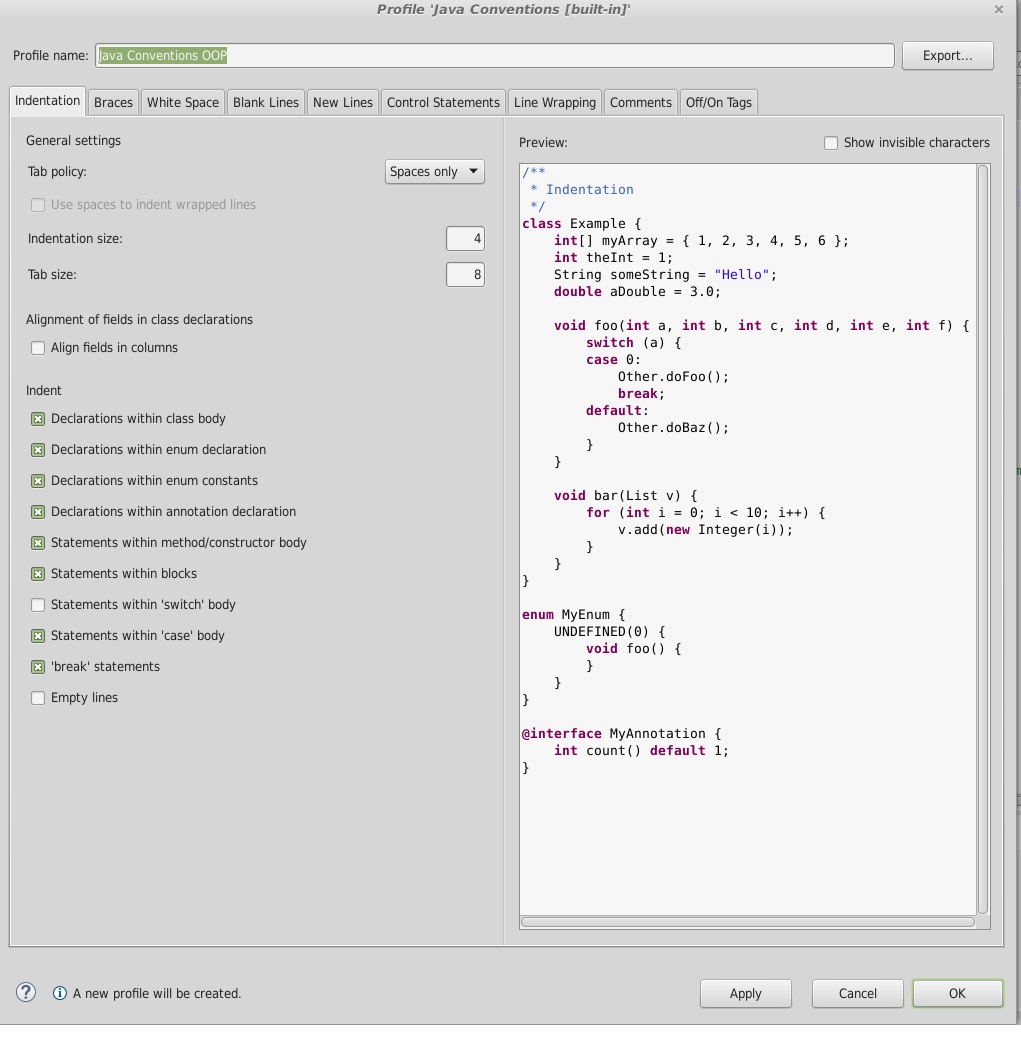
\includegraphics[width=0.99\textwidth]{img/ideconf-2}
}

\fr{Coding style: configurazione IDE Eclipse} {
	\centering
	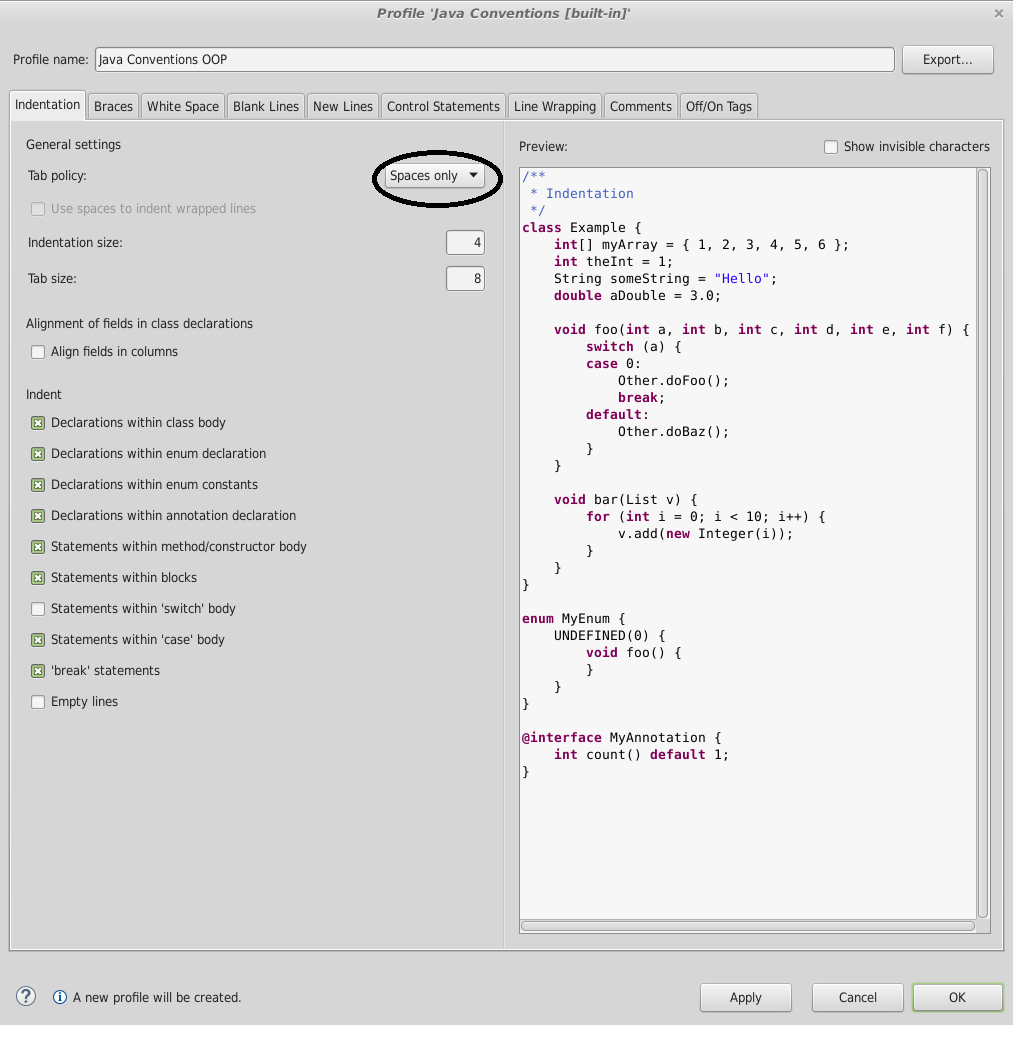
\includegraphics[width=0.99\textwidth]{img/ideconf-3}
}

\fr{Coding style: configurazione IDE Eclipse} {
	\centering
	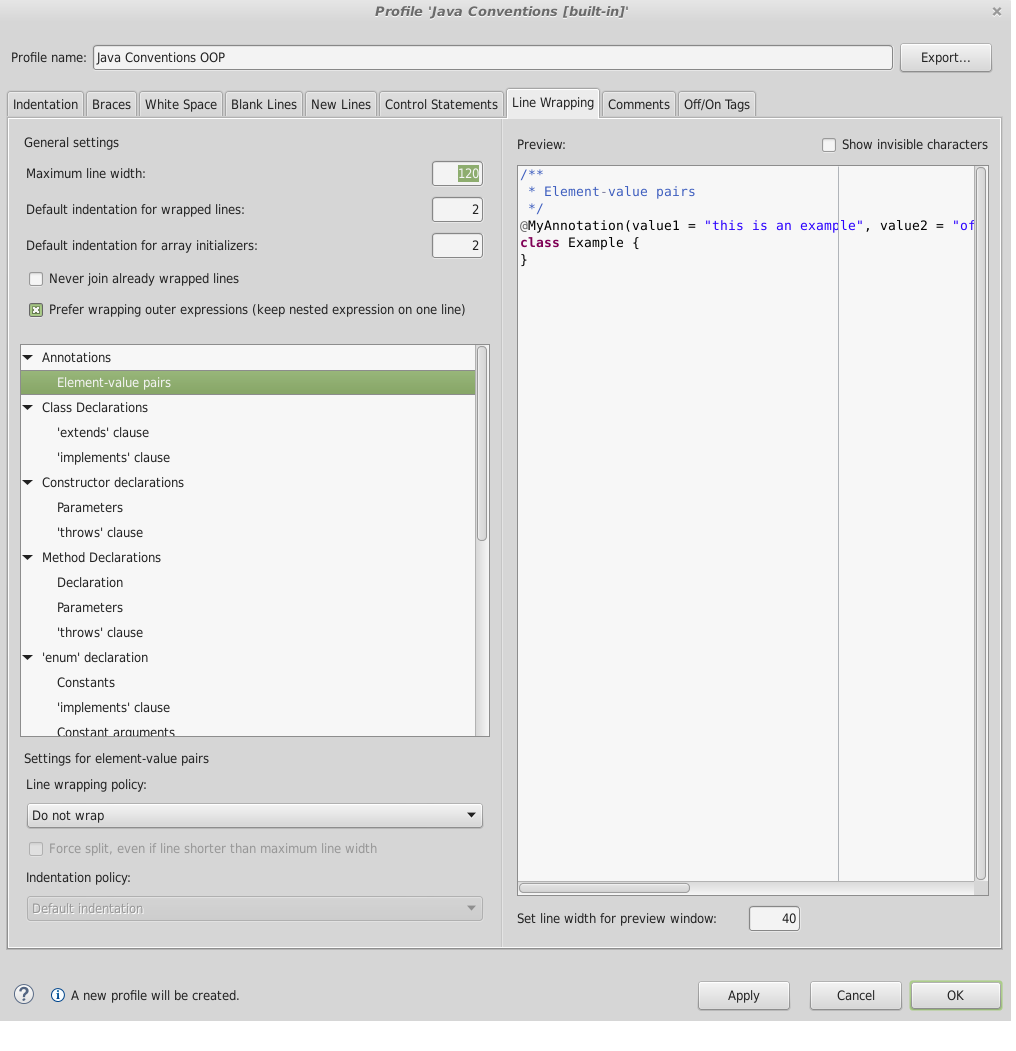
\includegraphics[width=0.99\textwidth]{img/ideconf-4}
}

\section{Esercitazione di oggi}
\fr{Preparazione Ambiente di Lavoro}{
  \iz{
    \item Accendere il PC
    \item Loggarsi sul sito del corso
    \iz{
      \item \textcolor{blue}{\moodleurl}
    }
    \item Scaricare dalla sezione \texttt{lab} del sito il file \texttt{lab06.zip} contenente il materiale dell'esercitazione odierna
    \item Spostare il file scaricato sul Desktop
    \item Decomprimere il file usando 7zip (o un programma analogo) sul Desktop
  }
}

\fr{Modalità di Lavoro}{
  \bl{}{
    \en{
      \item Gli esercizi sono divisi in package con nomi progressivi
      \item Troverete un commento con le istruzioni per ciascun esercizio
      \item Risolvere l'esercizio in autonomia
      \item Cercare di risolvere autonomamente eventuali piccoli problemi che possono verificarsi durante lo svolgimento degli esercizi
      \item \textcolor{red}{Utilizzare le funzioni di test presenti nei sorgenti per il testing dell'esercizio}
      \item Contattare i docenti nel caso vi troviate a lungo bloccati nella risoluzione di uno specifico esercizio
      \item \textbf{A esercizio ultimato contattare i docenti per un rapido controllo della soluzione realizzata}
      \item Proseguire con l'esercizio seguente
       \item \textcolor{red}{Generare il file JAR dell'intera esercitazione} (o in lab o a casa in mancanza di tempo)
    }
  }
}


\end{document}

